
\hypertarget{cv:registrarTray}{\section{Registrar Trayectoria}} \label{sec:registrarTray}

	Esta funcionalidad le permitirá registrar una trayectoria dentro del caso de uso que se esta operando.

		\subsection{Procedimiento}

			%Pasos de procedimiento
			\begin{enumerate}
	
			\item Oprima el botón \IURegistrar{} de la pantalla \ref{fig:GestionarTrayectorias} ''Gestionar Trayectorias''.
			
			\item Se mostrará la pantalla \ref{fig:registrarTray} ''Registrar Trayectoria''.

			%Pantalla
			\begin{figure}[H]
				\begin{center}
					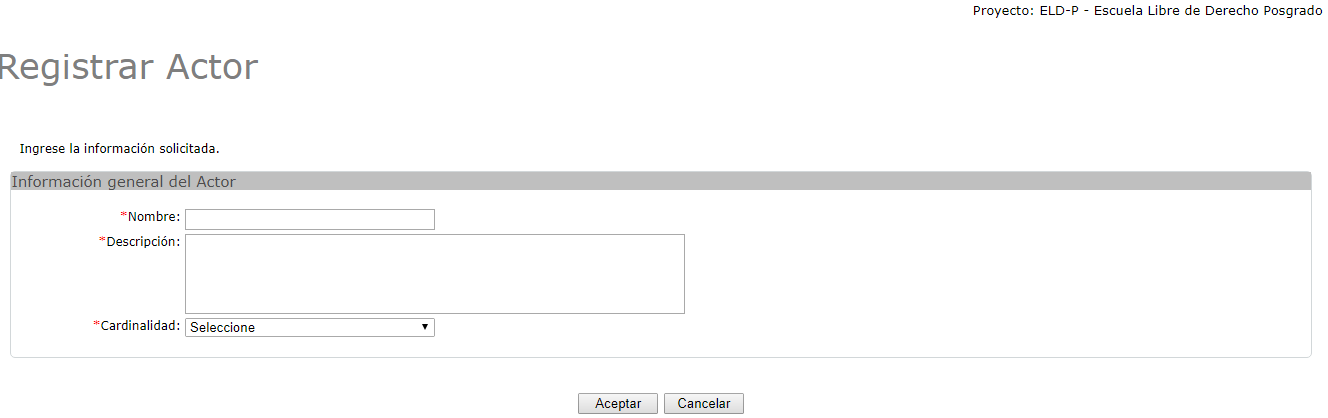
\includegraphics[scale=0.5]{roles/lider/actor/pantallas/IU10-1registrarActor}
					\caption{Registrar Trayectoria}
					\label{fig:registrarTray}
				\end{center}
			\end{figure}
		
			\item Ingrese una clave, el tipo de trayectoria que se esta registrando (principal o alternativa).
			
			\item En caso de registrar una trayectoria alternativa ingrese la condición correspondiente. 
			
			\item Oprima el botón \IUAceptar.
			
			\item Se mostrará el mensaje \ref{fig:trayRegistrada} en la pantalla \ref{fig:GestionarTrayectorias} ''Gestionar Trayectorias''.
			
			\begin{figure}[htbp!]
				\begin{center}
					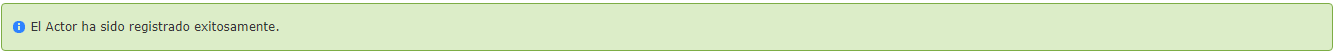
\includegraphics[scale=0.5]{roles/lider/actor/pantallas/IU10-1MSG1}
					\caption{MSG: Trayectoria Registrada}
					\label{fig:trayRegistrada}
				\end{center}
			\end{figure}
			\end{enumerate}